\chapter{Phase Transitions}

Phase Transitions are fundamental phenomena in statistical physics, where a system undergoes a qualitative change in its macroscopic properties as external parameters (like temperature or pressure) are varied. These transitions can be classified into different types based on their characteristics and the nature of the change in the system. Let us start from the definition of a phase of a many-particle system, which is crucial for understanding phase transitions.

\begin{definition}[Phase of Many-Particle System]
    A phase of a many-particle system is a region in the parameter space (e.g., temperature, pressure) where the system exhibits distinct physical properties and behavior: it is a ``type'' of collective state of matter. They are defined in terms of macroscopic properties such as density, magnetization, or symmetry.
\end{definition}

A phase transition occurs when a system undergoes an \textit{abrupt change from one phase to another} (states) \textit{as we smoothly vary an external parameter}. Often PTs are accompanied by a discontinuity or singularity in some thermodynamic quantity, which serves as an order parameter to characterize the transition.

A phase transition is always a result of a competition between ``order'' and ``disorder'' in the system. For example, in a ferromagnetic material, the ordered phase corresponds to a state where the magnetic moments are aligned, while the disordered phase corresponds to a state where the magnetic moments are randomly oriented. The transition between these two phases can be driven by temperature, where thermal fluctuations disrupt the order at high temperatures.

We are now going to define PTs in a mathematical framework, which will allow us to classify them into different types. To start we have to highlight how PTs are related to \textbf{singularities in the partition function} of the system at the thermodynamic limit, or equivalently in the free energy. The \textbf{free energy} is a thermodynamic potential that encodes the equilibrium properties of a system, and its behavior near a phase transition can reveal important information about the nature of the transition:
\[
    F = -\frac{1}{\beta} \ln Z = U - TS,
\]
where $Z$ is the partition function of the system and $\beta = 1/(k_B T)$ is the inverse temperature. A phase transition is typically associated with a non-analytic behavior of the free energy as a function of the external parameters, such as temperature or pressure. Thus PTs are defined as singularities in the thermodynamic limit of the partition function $Z$ or equivalently of the free energy $F$.

\begin{definition}[Phase Transition]
    A phase transition is a non-analytic behavior of the free energy $F$ as a function of external parameters (e.g., temperature, pressure) in the thermodynamic limit. This non-analyticity manifests as a discontinuity or singularity in some thermodynamic quantity, which serves as an order parameter to characterize the transition.
\end{definition}

\begin{example}[Finite system and phase transitions]
    If we consider a finite set of spins, the partition function $Z$ is a finite sum of exponentials, which is an analytic function of the parameters:
    \[
        Z = \sum_{\{\text{conf}\}} e^{- \beta E[\text{conf}]}.
    \]
    Therefore, in a finite system, there can be no true phase transition, as the free energy will always be analytic. However, as we take the thermodynamic limit (i.e., let the number of spins go to infinity), the partition function can develop singularities, leading to non-analytic behavior in the free energy and thus allowing for phase transitions to occur.
\end{example}

In physics we never encounter real infinite systems, but we can approximate them by considering large systems and taking the thermodynamic limit. This is a common approach in statistical mechanics to study phase transitions, as it allows us to capture the essential features of the transition while avoiding the complications that arise from finite-size effects.

\section{Classification of Phase Transitions}

Phase transitions can be classified into different types based on their characteristics and the nature of the change in the system. One of the first classifications was proposed by \textit{Paul Ehrenfest}, who categorized phase transitions based on the order of the derivative of the free energy that exhibits a discontinuity at the transition point. Today, we have a more refined classification, which is based on the concept of order parameters and symmetry breaking.

Phase transitions can be classified depending on the type of singularity in the free energy. We can distinguish between first-order and continuous (second-order) phase transitions:
\begin{itemize}
    \item \textbf{First-order phase transitions} are characterized by a discontinuity in the first derivative of the free energy with respect to some external parameter (e.g., temperature). This means that there is a \textbf{latent heat} associated with the transition, and the order parameter changes discontinuously.\footnote{This happens because we can express order parameters as derivatives of the free energy, which is continuous but has discontinuous first derivative.} Examples include the liquid-gas transition and the melting of a solid.
    \item \textbf{Continuous (second-order) phase transitions} are characterized by a continuous first derivative of the free energy, but a discontinuity in the second or higher derivatives. In this case, there is \textbf{no latent heat}, and the order parameter changes continuously. Examples include the ferromagnetic transition in the Ising model and the superconducting transition in certain materials. These are the most interesting PTs and will drive most of our discussion in the following chapters.
\end{itemize}
The latter group of PTs is also called \textbf{critical phenomena}, and they are associated with the emergence of long-range correlations and \textit{scale invariance} at the critical point. The study of critical phenomena has led to the development of powerful theoretical tools, such as the \textit{renormalization group}, which allows us to understand the universal behavior of systems near criticality.
Another important phenomenon associated with continuous phase transitions is the concept of \textbf{spontaneous symmetry breaking}. In many cases, the ordered phase of a system exhibits a lower symmetry than the disordered phase. This spontaneous symmetry breaking is a key feature of many continuous phase transitions and plays a crucial role in determining the properties of the system near criticality.

\subsection{Phase Diagram of Water}

Looking at the phase diagram of water, we can see that there are three main phases: solid (ice), liquid (water), and gas (vapor). The \textbf{phase boundaries} between these phases are represented by lines in the pressure-temperature (\(p\)-\(T\)) diagram, also called coexistence lines. The point where the liquid-gas phase boundary ends is called the \textbf{critical point}, which is a second-order phase transition (only ``crossing'' the specific point). Over this point, the properties of the liquid and gas phases become indistinguishable, suggesting that the two phases are not fundamentally different, and the system exhibits critical phenomena such as large fluctuations and long-range correlations.

\begin{figure}[H]
    \begin{minipage}{0.5\textwidth}
        Moving along the phase boundaries, we can observe first-order phase transitions, where the system undergoes a discontinuous change in density and other properties. For example, when water freezes into ice or boils into vapor, there is a latent heat associated with the transition, and the order parameter (density) changes discontinuously. The first derivative of the free energy with respect to temperature (which is related to the entropy) and pressure (which is related to the volume) will show a discontinuity at these transitions, confirming their first-order nature.
    \end{minipage}
    \hfill
    \begin{minipage}{0.45\textwidth}
        \centering
        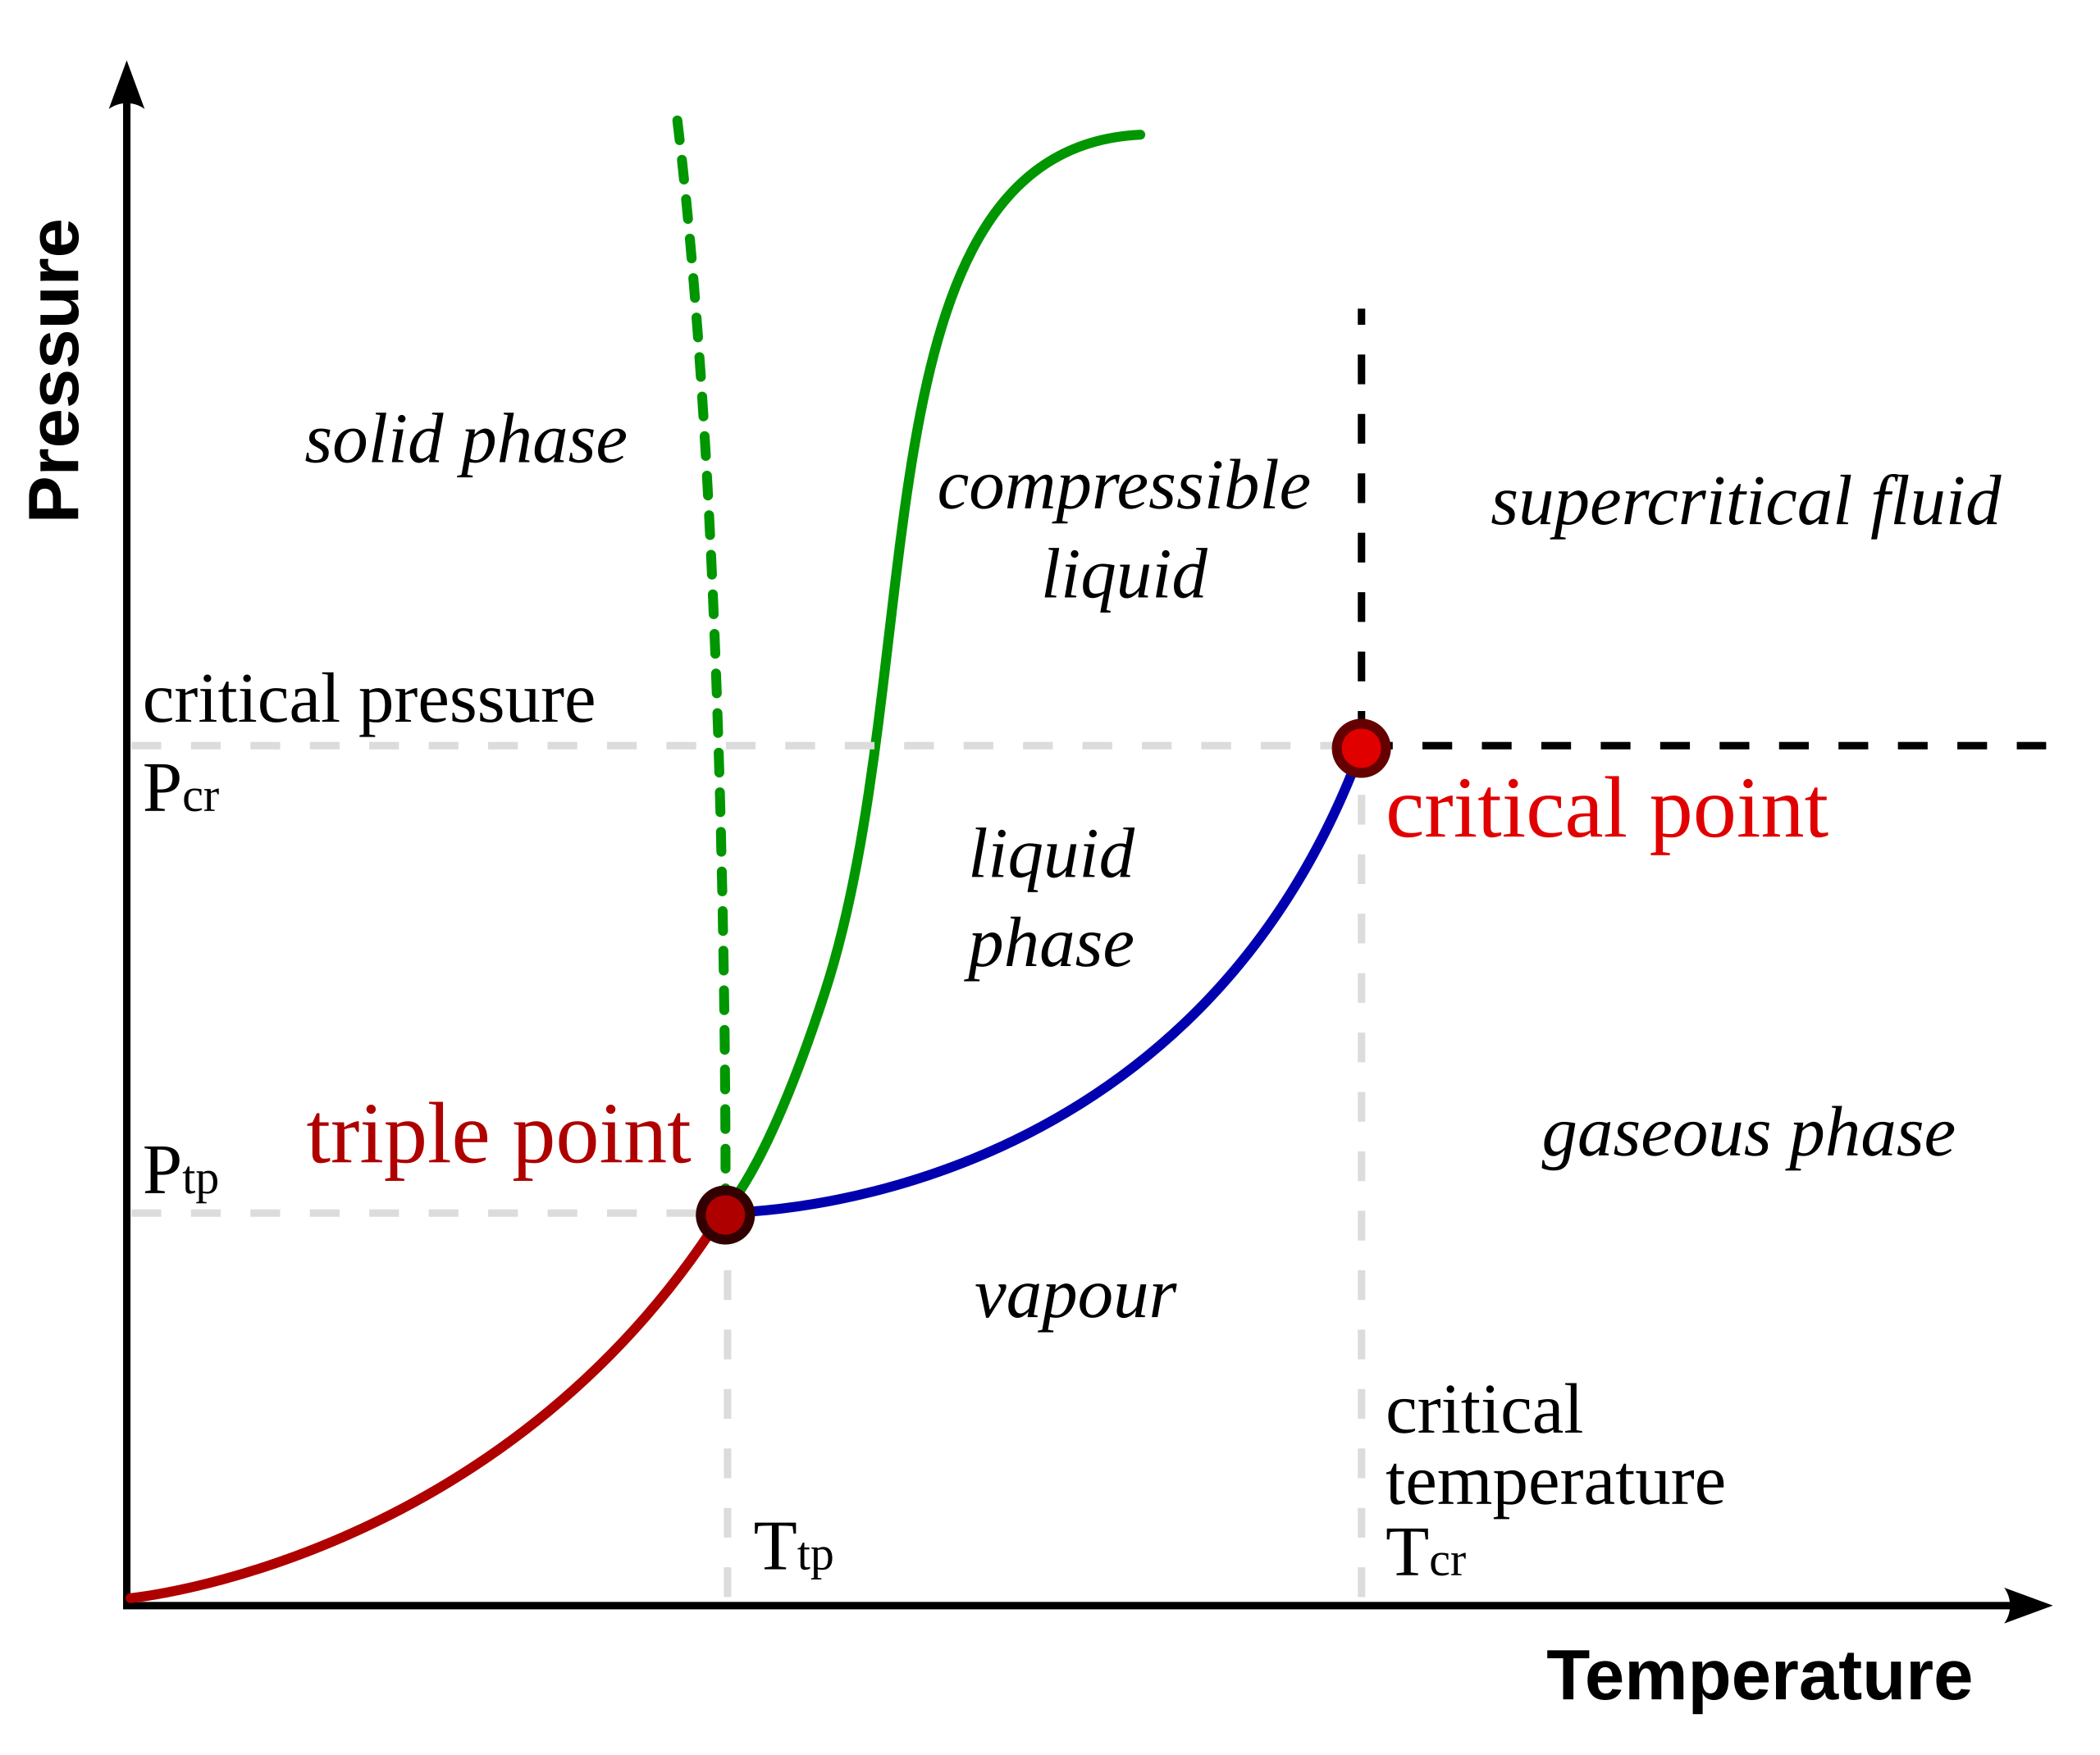
\includegraphics[width=\textwidth]{img/pt_water_diagram.png}

    \end{minipage}
    \centering
    \begin{minipage}{0.9\textwidth}
        \caption{Phase diagram of water in the pressure-temperature (\(p\)-\(T\)) plane. The lines represent the phase boundaries between solid, liquid, and gas phases, with the critical point marking the end of the liquid-gas phase boundary.}
    \end{minipage}
\end{figure}

Decreasing the pressure at a fixed temperature can also lead to phase transitions. For example, if we decrease the pressure of liquid water at a constant temperature, we can reach the point where it transitions into vapor. This is another example of a first-order phase transition, as there is a discontinuity in the density and other properties of the system.

Each point in the (\(p\)-\(T\)) phase diagram corresponds to a specific value of \(v = \frac{V}{N}\) specific volume, except for the points on the phase boundaries (I order transition lines), where we have a coexistence of phases and the specific volume can take on different values depending on the relative proportions of the coexisting phases. For example, along the liquid-gas phase boundary, we can have a mixture of liquid and gas phases, and the specific volume will depend on the ratio of liquid to gas in the mixture. This can be seen in the following phase diagram.

The phase diagram of water in the pressure-volume (\(p\)-\(v\)) plane shows indeed the different phases and the transitions between them, with the critical point marking the end of the liquid-gas phase boundary.

\begin{figure}[H]
    \begin{minipage}{0.5\textwidth}
        \centering
        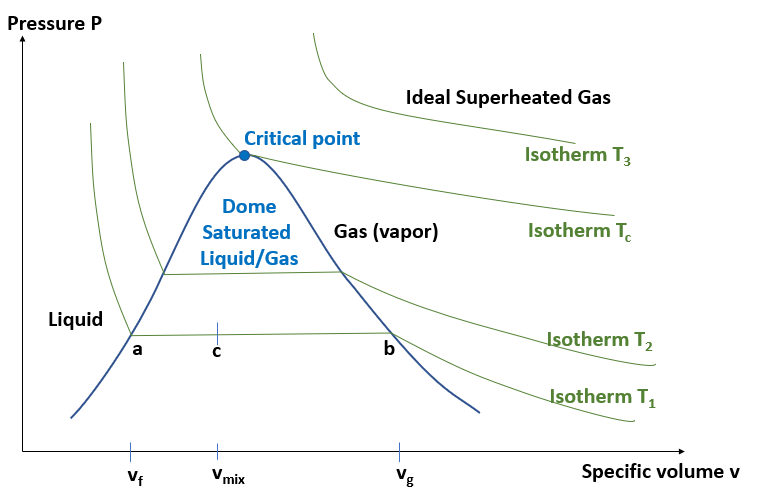
\includegraphics[width=\textwidth]{img/pv_water_diagram.png}
    \end{minipage}
    \hfill
    \begin{minipage}{0.45\textwidth}
        If we are below the critical temperature, at a fixed T we can observe all three phases by varying the pressure or volume: this isothermal lines form a mesoscopic domain where we can observe the coexistence of phases and the transitions between them. This is a rich area of study in statistical mechanics, as it allows us to explore the behavior of systems near criticality and understand the underlying mechanisms driving phase transitions.
    \end{minipage}
    \centering
    \begin{minipage}{0.9\textwidth}
        \caption{Phase diagram of a pure substance in the pressure-volume (\(p\)-\(v\)) plane. The lines represent the phase boundaries between different phases, with the critical point marking the end of the liquid-gas phase boundary.}
    \end{minipage}
\end{figure}

The isotherms in the previous diagram are not to be confused with the coexistence lines in the \(p\)-\(T\) diagram, which represent the phase boundaries. In the \(p\)-\(v\) diagram, the isotherms represent the behavior of the system at a fixed temperature as we vary the pressure and volume, and we encounter phase I order phase transitions as we cross the coexistence region (``dome'' of saturated liquid/gas). This region is characterized by a coexistence of liquid and gas phases, where the specific volume can take on different values depending on the relative proportions of the coexisting phases
\[
    \rho_g \sim \frac{1}{v_g}, \quad \rho_l \sim \frac{1}{v_l}, \quad \text{at } T<T_c.
\]
The critical point marks the end of this coexistence region, where the properties of the liquid and gas phases become indistinguishable.

The full phase diagram of water in the pressure-volume-temperature (\(p\)-\(v\)-\(T\)) space provides a comprehensive view of the different phases and the transitions between them. It shows how the phases of water change as we vary both temperature and pressure, with the critical point marking the end of the liquid-gas phase boundary.

\begin{figure}[H]
    \begin{minipage}{0.55\textwidth}
        \centering
        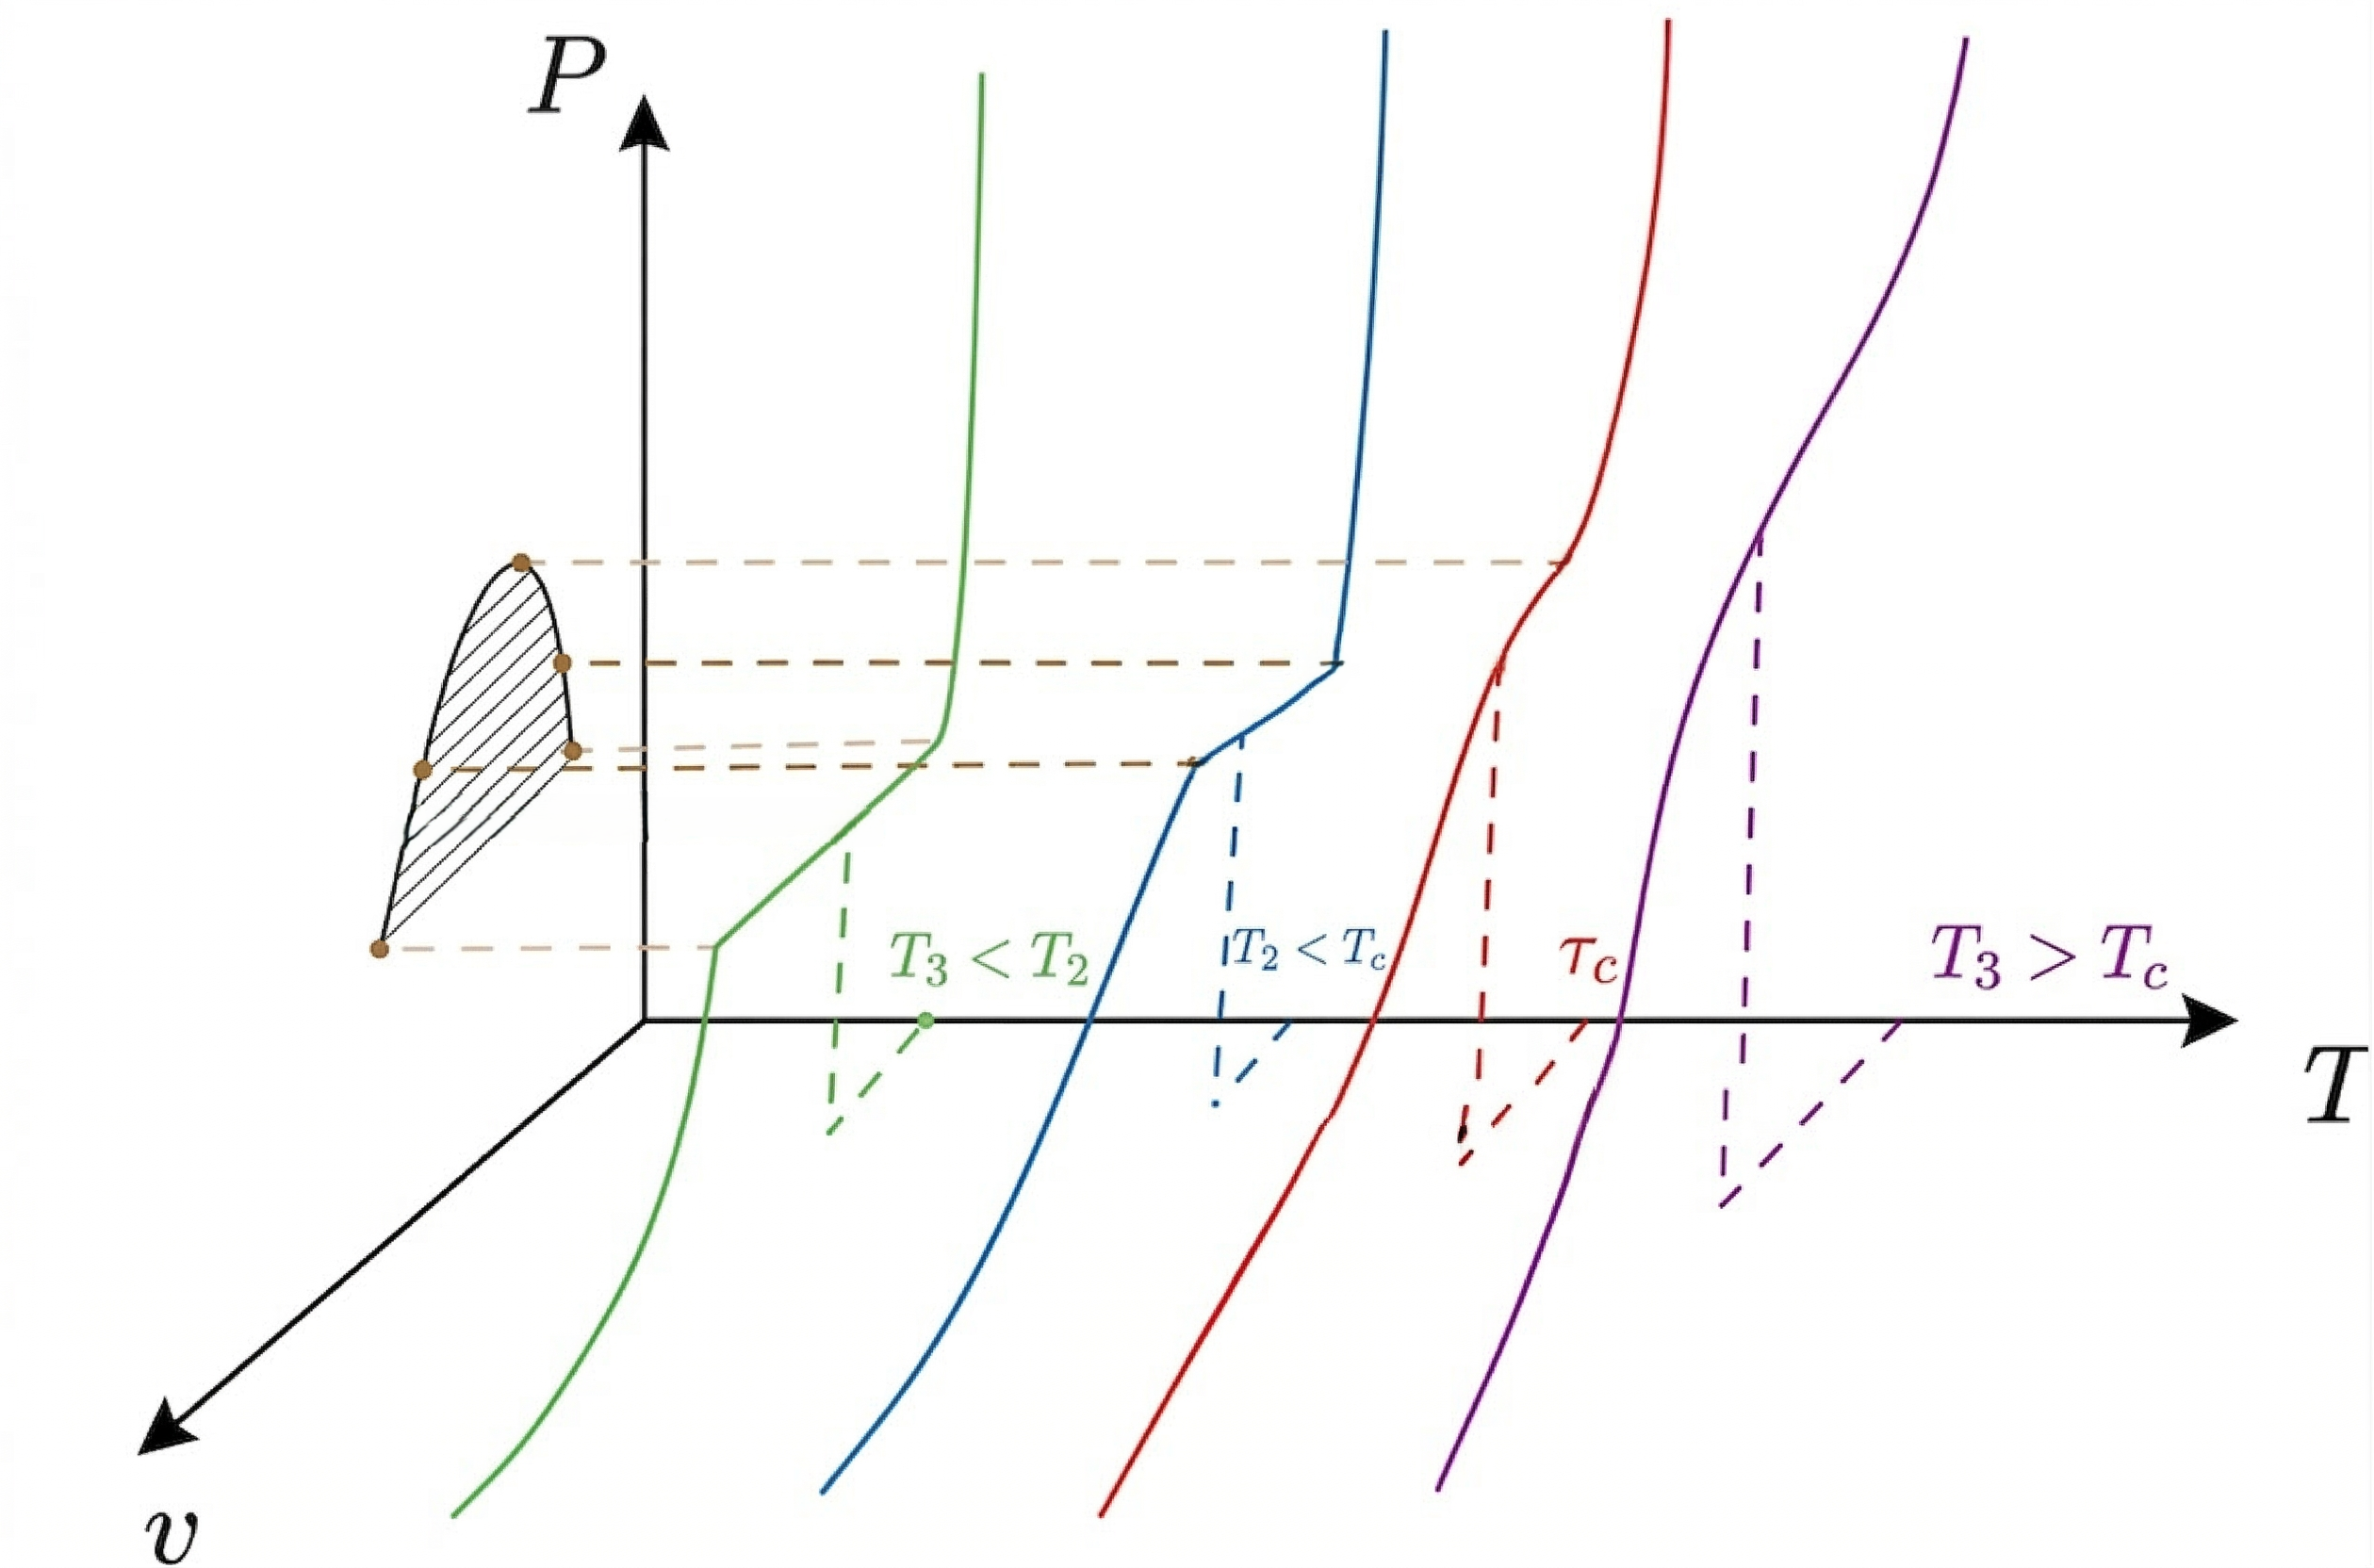
\includegraphics[width=0.85\textwidth]{img/pvt-water-diagram.png}
    \end{minipage}
    \hfill
    \begin{minipage}{0.4\textwidth}
        \centering
        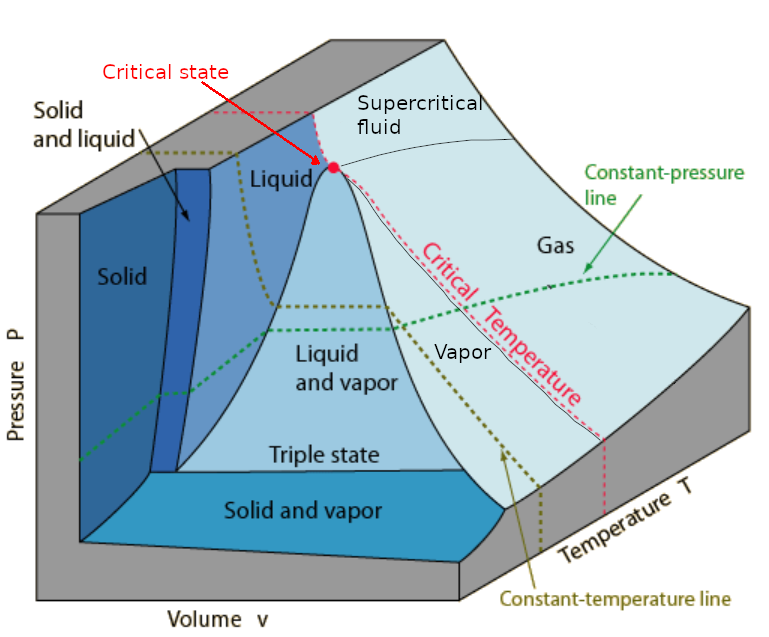
\includegraphics[width=\textwidth]{img/pvt_water_phase_diagram.png}
    \end{minipage}
    \centering
    \begin{minipage}{0.9\textwidth}
        \caption{Phase diagram of water in the pressure-volume-temperature (\(p\)-\(v\)-\(T\)) space. On the right, the surfaces represent the different phases of water, with the critical point marking the end of the liquid-gas phase boundary. On the left, different isotherms are shown, illustrating how the phases change as we vary temperature and pressure (only near the critical point).}
    \end{minipage}
\end{figure}

Transitions may be direction dependent in the phase space, meaning that the nature of the transition can change depending on the path taken in the parameter space. At the critical point, the system exhibits critical phenomena such as large fluctuations and long-range correlations. The properties of the system near the critical point can be described by critical exponents, which characterize how various physical quantities diverge or vanish as the critical point is approached. These critical exponents are universal, meaning that they depend only on the dimensionality of the system and the symmetry of the order parameter, rather than on the specific details of the microscopic interactions. This universality is a key feature of critical phenomena and allows us to classify different systems into universality classes based on their critical behavior.

Phase transitions are well defined when described with a curve in the parameter space, but we can also have transitions that occur at a single point, such as the critical point in the phase diagram of water. In this case, the transition is not associated with a curve but rather with a specific set of conditions (temperature and pressure) where the properties of the system change dramatically.

We are only going to discuss PTs which occurs with a smooth variation of the parameters, but there are also PTs that can occur with a sudden change in the parameters, such as a quench or a rapid cooling. These non-equilibrium phase transitions can lead to interesting phenomena such as the formation of topological defects and the emergence of new phases that are not present in equilibrium conditions. The study of non-equilibrium phase transitions is an active area of research in statistical mechanics and condensed matter physics.

\begin{remark}[Critical Opalescence]
    The \textbf{milky appearence} (or critical opalescence) of a system near the critical point is a direct consequence of the divergence of the correlation length \(\xi\) (for example in a liquid-gas mixture). As the correlation length increases, fluctuations in the density or order parameter occur over larger and larger distances, leading to the scattering of light and giving rise to a milky or cloudy appearance. This phenomenon is a visual manifestation of the critical behavior of the system and is often observed in fluids near their critical point, such as in the case of water at its critical temperature and pressure.
\end{remark}

\subsection{Magnetic System}

In this setting, we are considering a universal magnetic system, which can be described by a Hamiltonian that includes interactions between magnetic moments (spins) and an external magnetic field. The behavior of the system can be analyzed in terms of its phase transitions, which are characterized by changes in the order parameter (magnetization) as we vary the temperature and the external magnetic field.

We have few control parameters over the system: the temperature $T$ and the external magnetic field $h$. The phase diagram of the magnetic system can be represented in the $T-h$ plane, where we can identify different phases based on the behavior of the magnetization.

\begin{figure}[H]
    \begin{minipage}{0.6\textwidth}
        \centering
        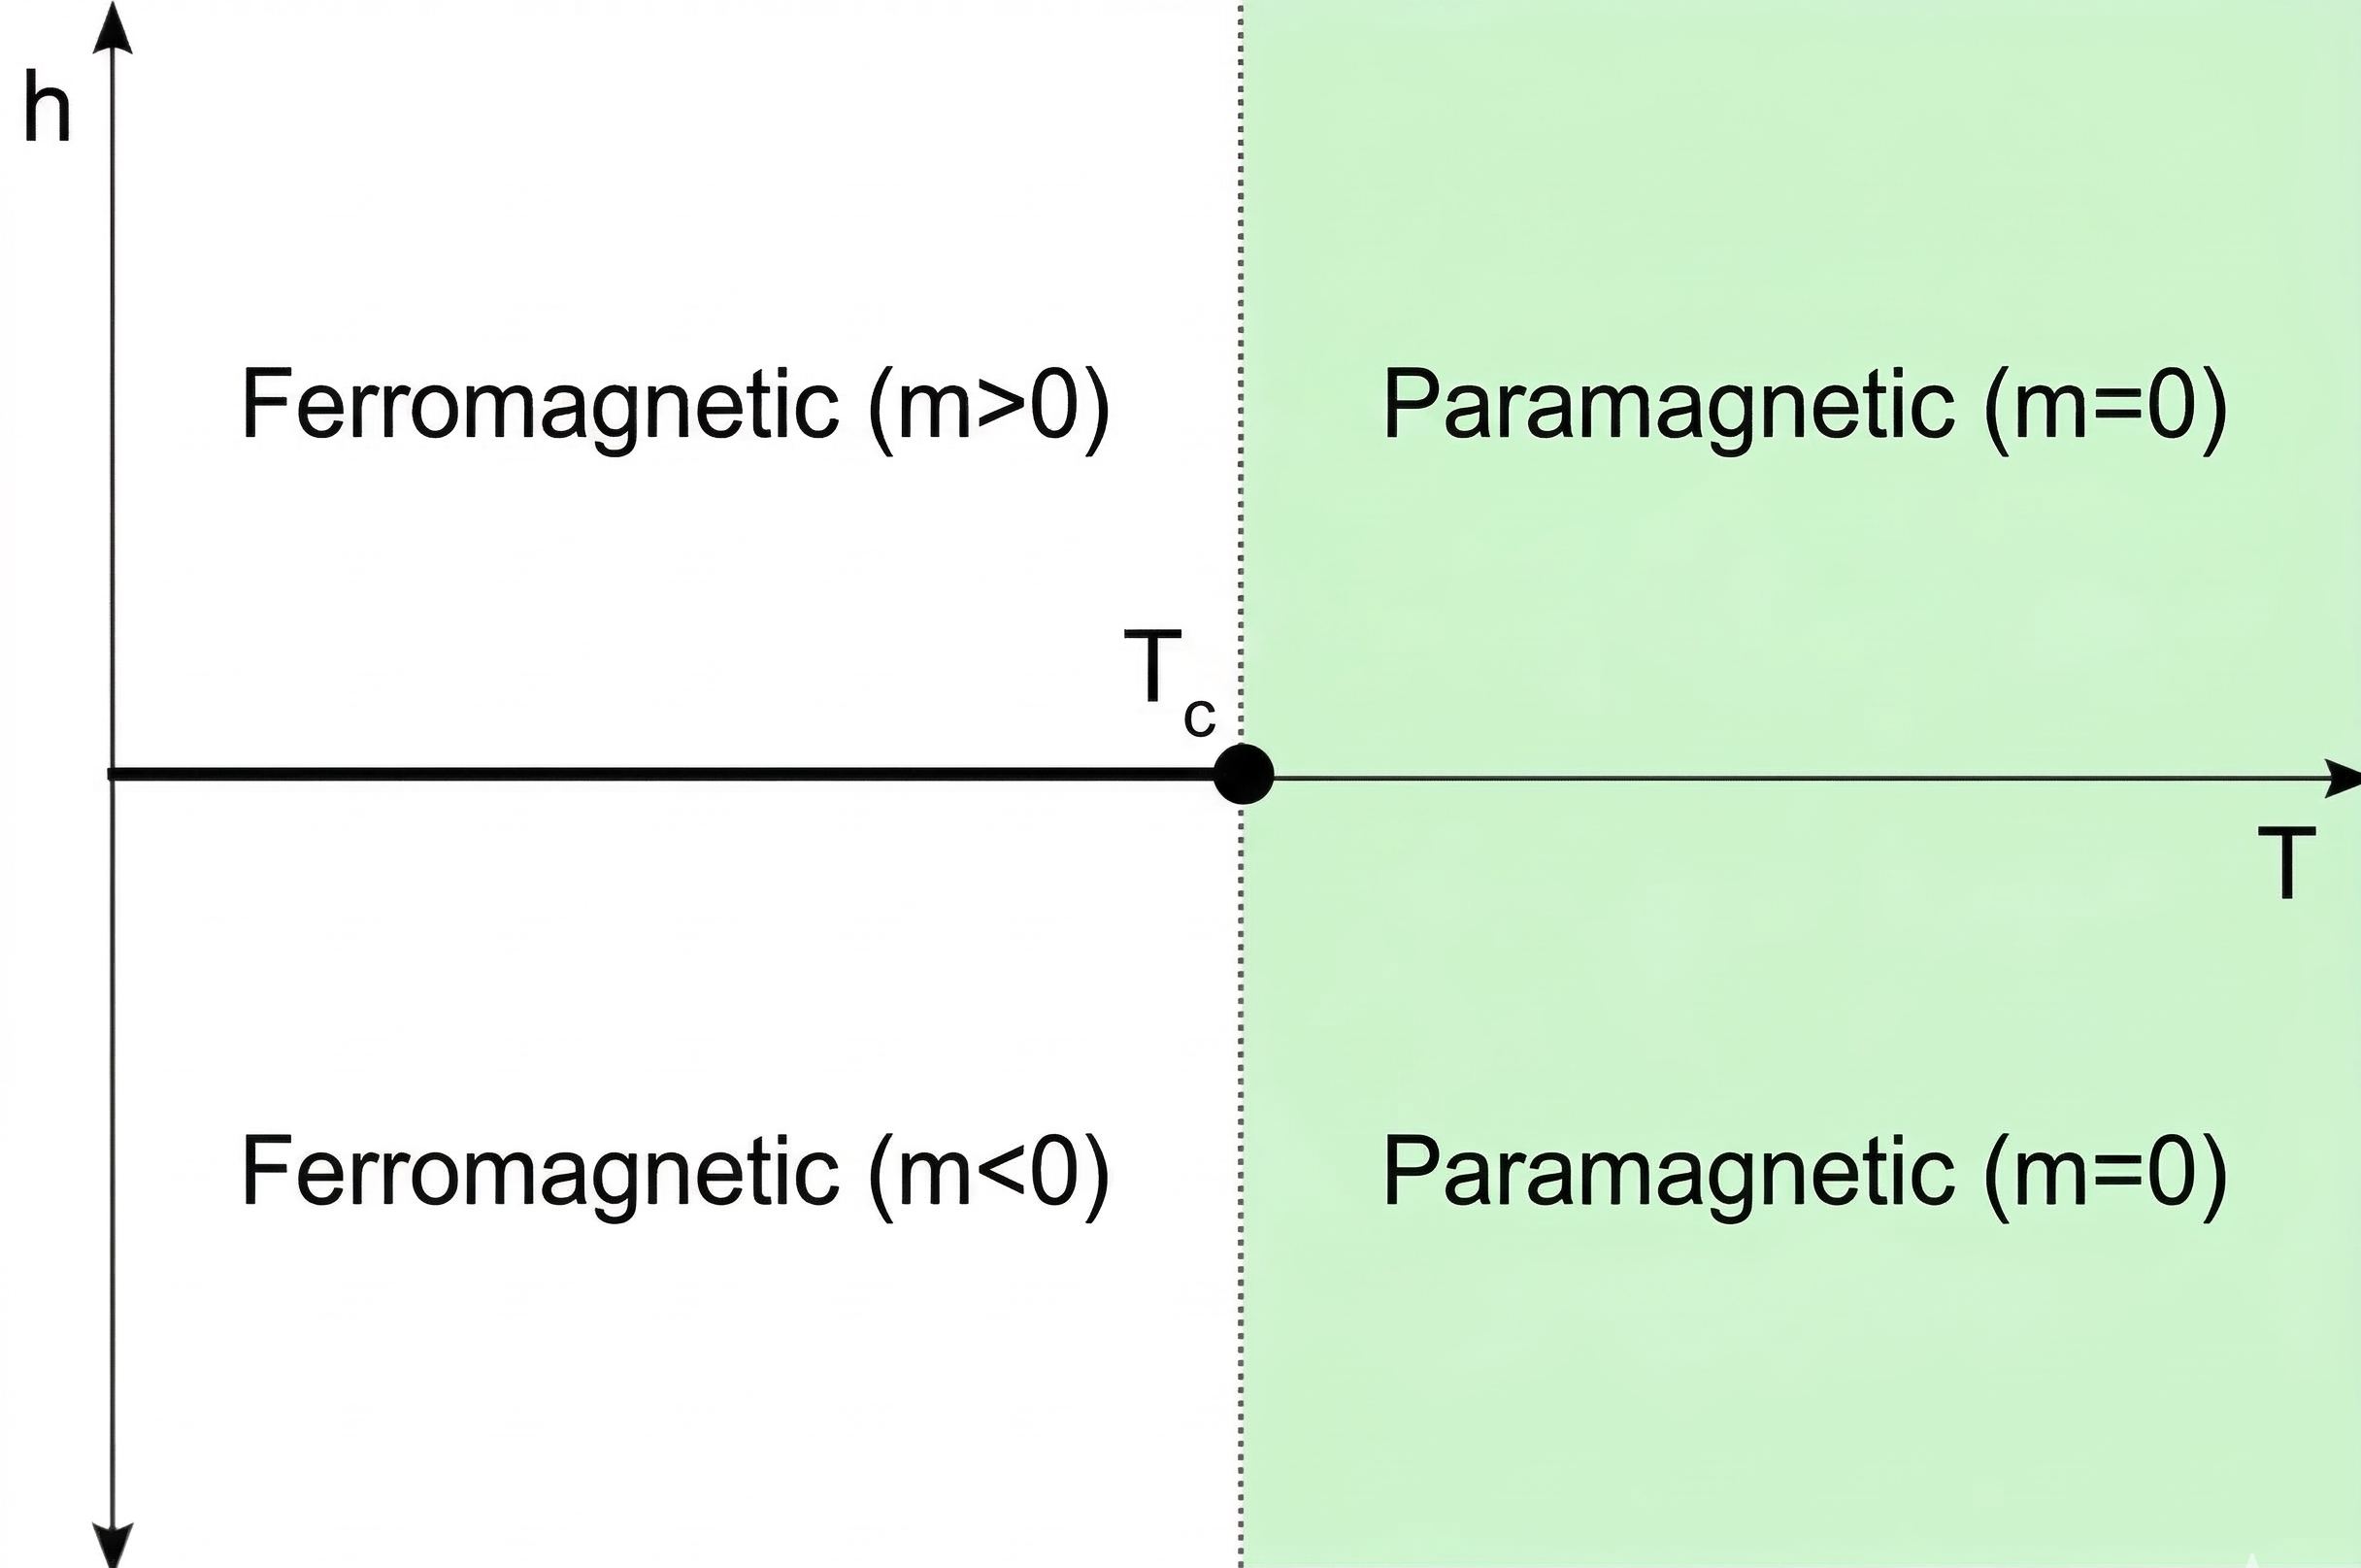
\includegraphics[width=0.8\textwidth]{img/h-T_phase_diagram.png}
    \end{minipage}
    \hfill
    \begin{minipage}{0.35\textwidth}
        \caption{Phase diagram of a magnetic system in the (\(h\)-\(T\)) plane, showing the ferromagnetic phase at low temperatures, cut in half by the first-order phase transition line, which ends at the critical point. Over the critical point, the system is in the paramagnetic phase.}
    \end{minipage}
\end{figure}

\begin{itemize}
    \item At high temperatures and low magnetic fields, the system is in a disordered phase where the magnetization is zero: \textbf{paramagnetic phase}.
    \item At low temperatures and high magnetic fields, the system is in an ordered phase where the magnetization is non-zero: \textbf{ferromagnetic phase}.
    \item The transition between these two phases can be either first-order or second-order, depending on the specific interactions in the system. If we cross the phase buondary under the critical point, we observe a first-order phase transition, while if we cross the critical point, we observe a second-order phase transition. Over it we have only the paramagnetic phase, which is a disordered phase with zero magnetization.
    \item At the critical point, the system exhibits critical phenomena such as large fluctuations in magnetization and long-range correlations. The properties of the system near the critical point can be described by critical exponents, which characterize how various physical quantities diverge or vanish as the critical point is approached.
\end{itemize}

Introducing the \textbf{magnetization} as the order parameter of the system, we can analyze how it changes across the phase transitions.

\begin{definition}[Order Parameter]
    An order parameter is a quantity that serves as a measure of the degree of order in a system and can be used to characterize different phases. It typically takes on a non-zero value in the ordered phase and vanishes in the disordered phase. It is expressed generally as
    \[
        m(T) = \frac{1}{V} \lim_{h \to 0} \langle M(h,T) \rangle,
    \]
    where the notation is deliberately describing the case of magnetization, but we can interpret more generally as the order parameter of a system, which can be defined in terms of the expectation value of some observable that characterizes the order in the system.

    Thus we interpret in general as
    \[
        \phi(T) = \frac{1}{V} \lim_{h \to 0} \langle O(h,T) \rangle,
    \]
    where $O(h,T)$ is an observable that characterizes the order in the system, and $V$ is the volume of the system, \(h\) is an external field that couples to the order parameter, and the limit \(h \to 0\) ensures that we are measuring the spontaneous magnetization (or order parameter) in the absence of an external field.
\end{definition}

In the paramagnetic phase, the magnetization is zero, while in the ferromagnetic phase, it takes on a non-zero value. The behavior of the magnetization near the critical point can be described by a power law, with a critical exponent that characterizes how the magnetization vanishes as we approach the critical point from the ordered phase.

\begin{figure}[H]
    \begin{minipage}{0.35\textwidth}
        \caption{Phase diagram of a magnetic system in the (\(M\)-\(h\)) plane, showing the behavior of the magnetization as an order parameter as a function of the external magnetic field at different temperatures. The coexistence line at the critical temperature is shown.}
    \end{minipage}
    \hfill
    \begin{minipage}{0.6\textwidth}
        \centering
        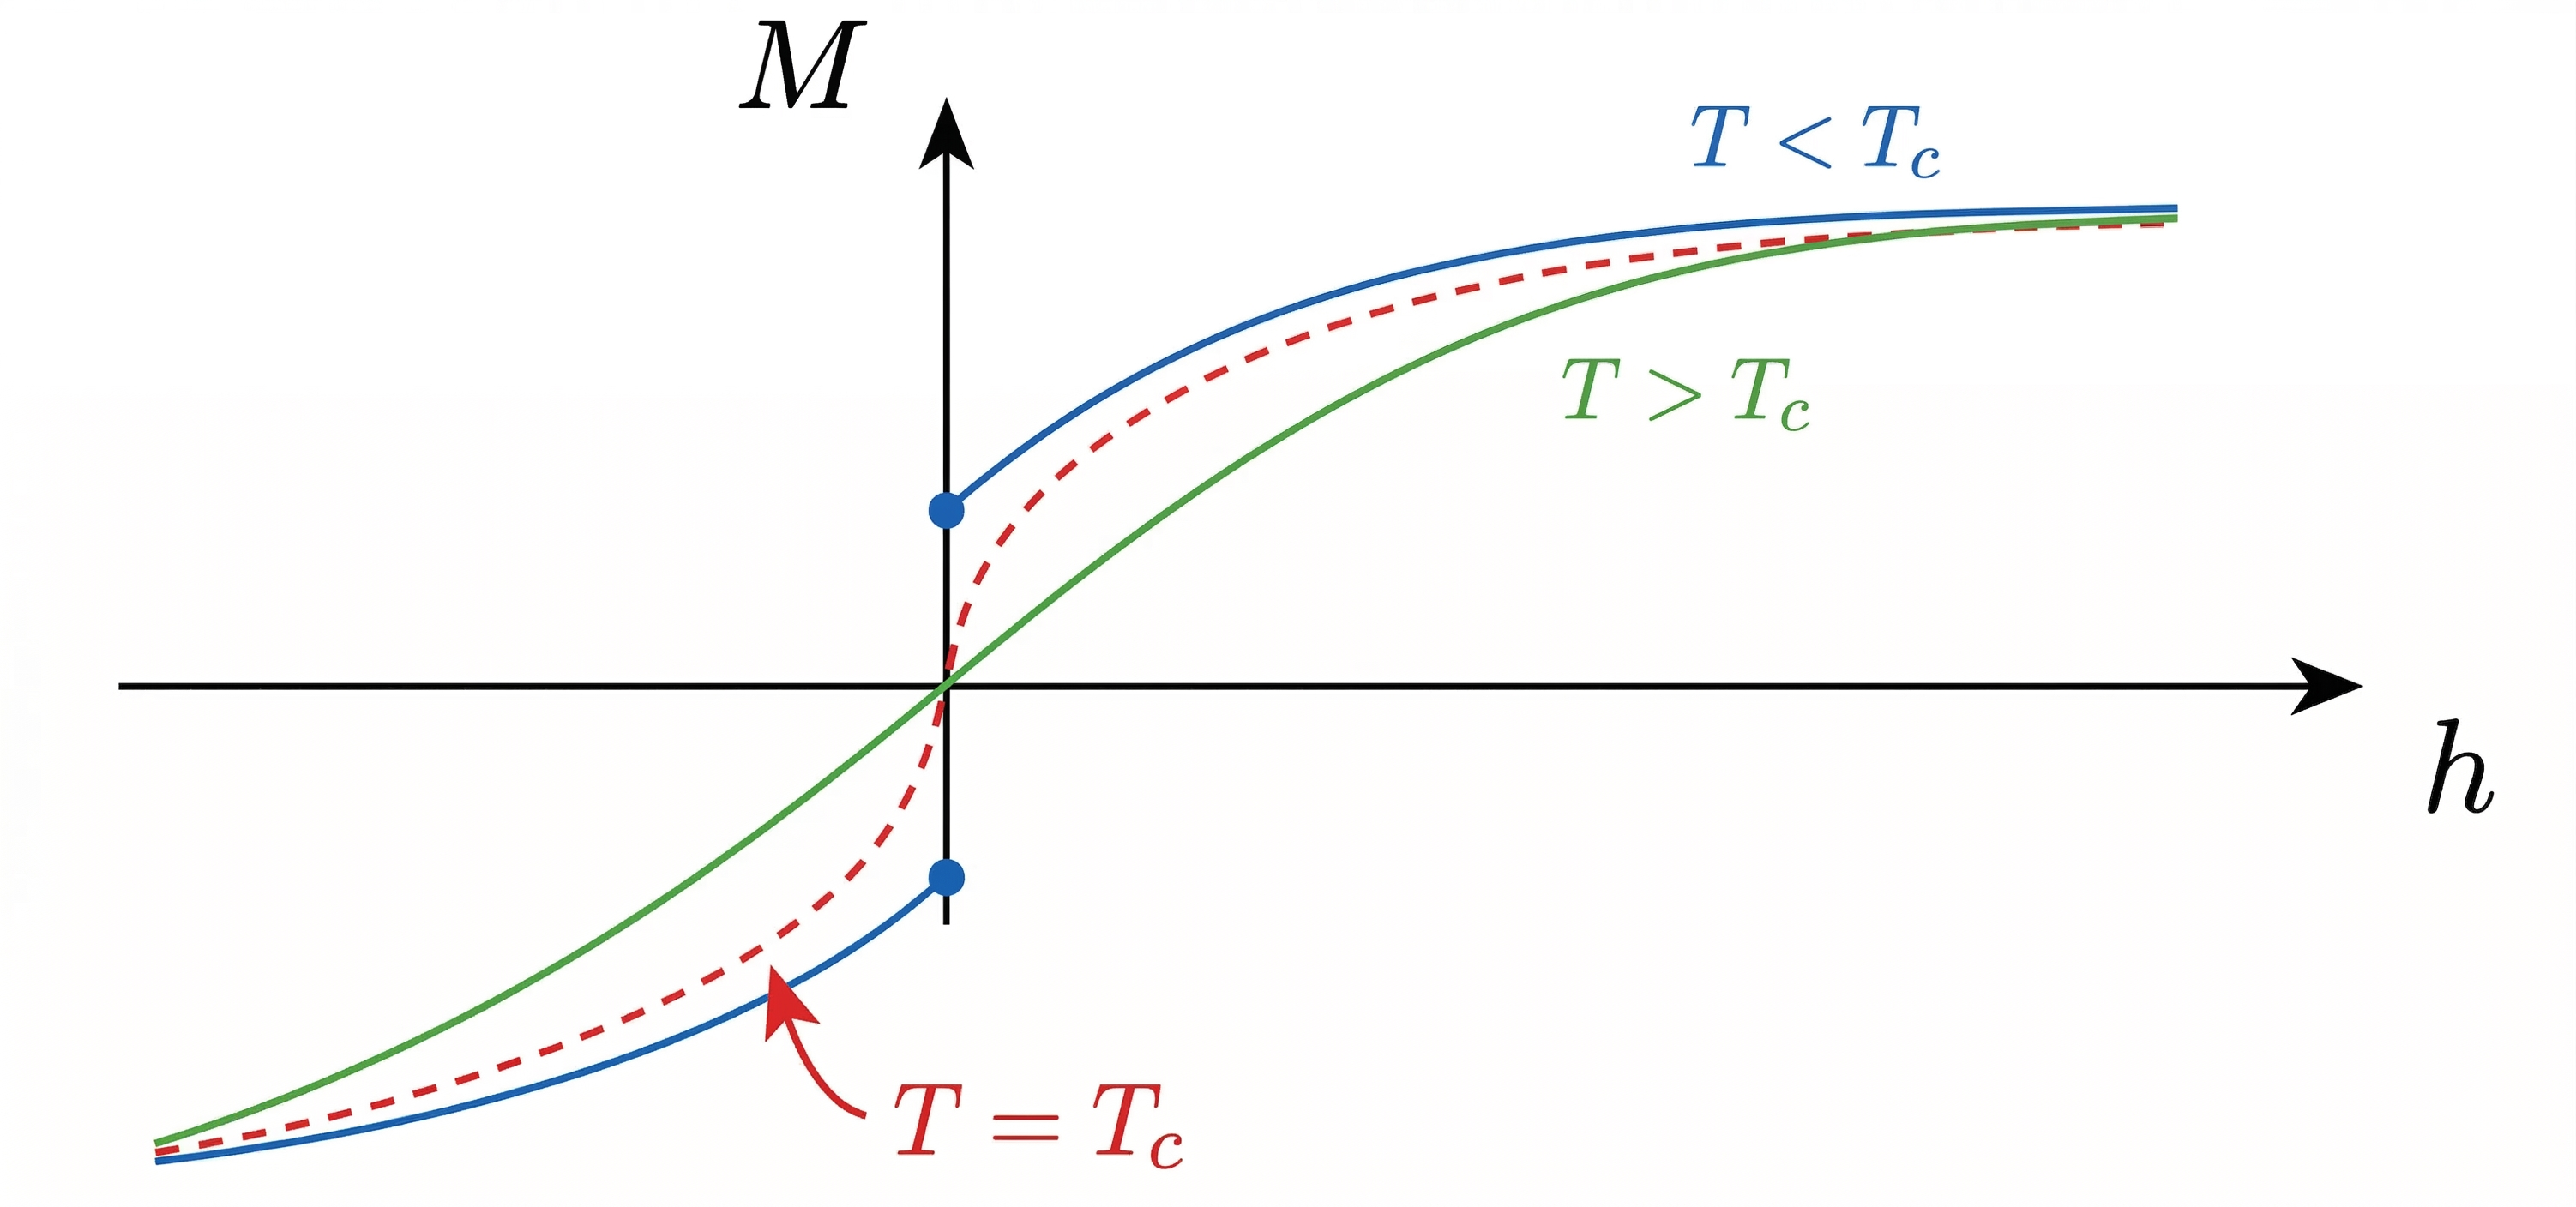
\includegraphics[width=0.9\textwidth]{img/M-h_phase_diagram.png}
    \end{minipage}
\end{figure}

This is equivalent to the jump of the volume in the liquid-gas transition (p-v water diagram), which is the order parameter of that system. Indeed, the red line in the previous figure represents the coexistence line, where the system can exist in both phases. The magnetization serves as a measure of the degree of order in the magnetic system, and it is associated to a first derivative of the free energy, which is discontinuous at a first-order phase transition and continuous at a second-order phase transition.

At any temperature below the critical temperature, we can observe a first-order phase transition by varying the external magnetic field. As we increase the magnetic field from zero, the system transitions from the paramagnetic phase to the ferromagnetic phase, with a discontinuous change in magnetization. This is a first-order phase transition, as there is a latent heat associated with the transition and the order parameter (magnetization) changes discontinuously.

The critical temperature separates two phases with different symmetries: the paramagnetic phase has a higher symmetry (rotational symmetry) than the ferromagnetic phase (which has a lower symmetry due to the alignment of spins). This is an example of spontaneous symmetry breaking, where the ordered phase exhibits a lower symmetry than the disordered phase. The study of this magnetic system and its phase transitions provides valuable insights into the behavior of many other systems that exhibit similar phenomena, such as superconductors and liquid crystals.

\subsection{Critical Behaviour}

When the order parameter approaches zero continuously at the critical point, we can describe its behavior using a power law:
\[
    m(T) = \begin{dcases}
        0               & \text{for } T > T_c, \\
        (T_c - T)^\beta & \text{for } T < T_c,
    \end{dcases}
\]
where $\beta$ is the critical exponent that characterizes how the magnetization vanishes as we approach the critical point from the ordered phase. The value of $\beta$ depends on the universality class of the system, which is determined by factors such as the dimensionality of the system and the symmetry of the order parameter. For example, in the three-dimensional Ising model, which is a prototypical model for ferromagnetic phase transitions, the critical exponent $\beta$ is approximately 0.326.

The surprising thing is that if we compute the same exponent for a completely different system, such as the liquid-gas transition, using some difference in densities as the order parameter, we find the same value of $\beta$:
\[
    \begin{dcases}
        \vert \rho_l - \rho_c \vert \sim (T - T_c)^\beta, \\
        \vert \rho_c - \rho_g \vert \sim (T - T_c)^\beta,
    \end{dcases} \quad \beta \approx 0.326,
\]
where $\rho_l$ and $\rho_g$ are the densities of the liquid and gas phases, respectively, \(\rho_c\) at the critical point, and the critical exponent $\beta$ is exactely the same as in the magnetic system, despite the fact that these systems have different microscopic details and interactions.

This is a manifestation of the \textbf{universality of critical phenomena}, which states that systems with different microscopic details can exhibit the same critical behavior near the phase transition, as long as they belong to the same universality class. This universality allows us to classify different systems based on their critical exponents and understand their behavior near criticality without needing to know the specific details of their interactions.

\subsection{Critical Exponents and Universality Classes}

The critical exponents are a set of numbers that characterize the behavior of physical quantities near the critical point. They describe how various properties of the system diverge or vanish as the critical point is approached. Some of the most common critical exponents include:
\begin{itemize}
    \item $\beta$: describes the behavior of the \textbf{order parameter} \textit{as a function of temperature} near the critical point, $m(T) \sim (T_c - T)^\beta$ for $T < T_c$. We have already discussed this exponent in the context of the magnetization and the liquid-gas transition, where it characterizes how the order parameter vanishes as we approach the critical point from the ordered phase.
    \item $\alpha$: describes the divergence of the specific heat (heat capacity) at constant volume and zero external field as a function of temperature near the critical point,
          \[
              C_V \sim |T - T_c|^{-\alpha},
          \]
          and the heat capacity is defined as the second derivative of the free energy with respect to temperature:
          \[
              C_V = \frac{\partial U}{\partial T} = \frac{\partial}{\partial T} (F + TS) = T \frac{\partial S}{\partial T} = -T \frac{\partial^2 F}{\partial T^2}.
          \]
          If we denote by \(c_\pm(T,h=0)\) the heat capacity at zero external field above/below the critical point (\(t = \tfrac{T-T_c}{T_c}\)), we can express the critical behavior of the heat capacity as
          \[
              c_\pm(t, h=0) \sim |t|^{-\alpha_\pm},
          \]
          where \(\alpha_\pm\) are the critical exponents for the heat capacity, in principle different above and below the critical point.
    \item $\delta$: describes the behavior of the \textbf{order parameter} \textit{as a function of the external field} at the critical temperature,
          \[
              m(h) \sim h^{1/\delta} \quad \text{at } T = T_c,
          \]
          where $h$ is the external magnetic field. This means that the magnetization, along the critical isotherm, behaves as a power law in the external field, going to zero as the field goes to zero with the previus dependence on \(\delta\).
    \item $\gamma$: describes the divergence of the \textit{zero-field} \textbf{susceptibility} \textit{as a function of temperature}:
          \[
              \chi \sim |T - T_c|^{-\gamma},
          \]
          where the susceptibility $\chi$ is defined as the derivative of the order parameter with respect to the external field:
          \[
              \chi_\pm = \chi(t \to 0^{\pm}) = \left(\frac{\partial m}{\partial h}\right)_{h=0}, \quad \chi_\pm \sim |t|^{-\gamma_{\pm}},
          \]
          with $t = (T - T_c)/T_c$ being again the reduced temperature. The susceptibility measures how responsive the system is to changes in the external field, and its divergence at the critical point indicates that even a small change in the magnetic field can lead to a large change in the magnetization. This is a hallmark of criticality and is associated with the emergence of long-range correlations in the system.

\end{itemize}

\subsubsection{Correlation Length and Universality}

Before continuing with the definitions of \(\nu\) and \(\eta\), we have to introduce the concept of \textbf{correlation length}, which is a measure of how far correlations in the system extend. Near the critical point, the correlation length diverges, indicating that fluctuations occur over increasingly large distances. Let us introduce it through a little model: let us consider a system of spins on a lattice, where each spin \(s_i\) can take on values of +1 or -1.
The magnetization \(m\) is defined as the average spin per site:
\[
    m = \frac{1}{N} \sum_{i=1}^N \langle s_i \rangle,
\]
where the angle brackets denote the thermal average:
\[
    \langle s_i \rangle = \mathbb{E}_{c}\left[ s_i \right]  = \frac{1}{Z} \sum_{\{s_k\}} s_i e^{-\beta H(\{s_k\},h)},
\]
with \(Z\) being the partition function and \(H\) the Hamiltonian of the system. The correlation function \(G(r)\) is defined as the average relative alignment of spins, i.e. the average product of spins at a distance \(r\):
\[
    G^{(2)}_{ij} = \langle s_i s_j \rangle = \frac{1}{Z} \sum_{\{s_k\}} s_i s_j e^{-\beta H(\{s_k\},h)} = G^{(2)}(\mathbf{r}), \quad \text{where } \mathbf{r} = \vert \mathbf{r}_i - \mathbf{r}_j \vert.
\]
Since \(G_{ij}^{(2)}\) depends only on the distance between spins for translational invariance, it depends only on the distance \(r\). We can then define the \textbf{connected correlation function}, which measures the correlations between fluctuations in the system:
\[
    G_c^{(2)}(\mathbf{r}) = \langle \left(s_i - \langle s_i \rangle\right) \left(s_j - \langle s_j \rangle\right) \rangle = \langle s_i \rangle \langle s_j \rangle - \langle s_i \rangle \langle s_j \rangle.
\]
The correlation length \(\xi\) is defined as the characteristic length scale over which correlations decay in the system, away from the critical point:
\[
    G_c^{(2)}(\mathbf{r}) \sim e^{- r/\xi} \quad \text{for } r \gg \xi.
\]
Near the critical point, the correlation function typically decays as a power law, which can be described by the critical exponent \(\eta\). Let us introduce two more critical exponents describing the behavior of the correlation function and the correlation length near the critical point:
\begin{itemize}
    \item $\nu$: describes the divergence of the correlation length, $\xi_{\pm} \sim |T - T_c|^{-\nu_{\pm}}$, with \(\nu_{\pm}>0\).
    \item $\eta$: describes the behavior of the correlation function at the critical point, $G(r) \sim r^{-(d-2+\eta)}$ at $T = T_c$, where $d$ is the dimensionality of the system.
\end{itemize}

\begin{remark}[Critical Opalescence and Correlation Length]
    Going back to the phenomenon of critical opalescence, we can understand it better after having introduced the correlation length. Since the wavelength of visible light is much larger than the microscopic length scales of the system (i.e. atomic distances), the scattering of light must be related to density fluctuations that occur over large distances. Near the critical point, the correlation length diverges, which means that fluctuations occur over increasingly large distances. This leads to a significant scattering of light, giving rise to the milky or cloudy appearance known as critical opalescence. When the correlation length diverges, the system becomes increasingly sensitive to fluctuations, and exhibits macroscopic collective behavior that allow us to ignore the microscopic details of the system and focus on the universal properties that emerge near criticality.
\end{remark}

Now we are ready to define and discuss the concept of \textbf{universality classes}. Systems that share the same critical exponents and scaling behavior near the critical point are said to belong to the same universality class. The universality class of a system is determined by factors such as the dimensionality of the system, the symmetry of the order parameter, and the range of interactions between particles.

\begin{definition}[Universality Class]
    A universality class is a category of systems that share the same critical exponents and scaling behavior near the critical point, regardless of their microscopic details. Systems that belong to the same universality class exhibit the same critical behavior and can be described by the same effective field theory near the critical point. The universality class of a system is determined by factors such as the dimensionality of the system, the symmetry of the order parameter, and the range of interactions between particles.
\end{definition}

Let us now make some observations about the critical behavior of systems near phase transitions, which will be important for our understanding of critical phenomena and the renormalization group.

\begin{remark}
    There is a connection between the divergence of the correlation length the response funcion. \TODO{add reference to Kardar - stat ph of fields, 1.4}
    The connection relies on the fact that near the critical point, the system exhibits long-range correlations, which means that fluctuations occur over increasingly large distances. This leads to a divergence in the correlation length \(\xi\), which in turn causes the response function (such as susceptibility) to diverge as well.
\end{remark}

The response function measures indeed how the system responds to external perturbations, and its divergence at the critical point indicates that even a small change in the external field can lead to a large change in the order parameter, which is a hallmark of criticality.

\begin{remark}\TODO{add reference to J. Cardy - scaling and renormalization in statistical physics, 1.2}
    Second order phase transitions are also called \textbf{continuous phase transitions} because the order parameter changes continuously across the transition, and there is no latent heat associated with the transition. As we will see, these PTs are associated with the \textbf{spontanoeus symmetry breaking}. In some cases, the symmetry is only \textbf{emergent}, meaning that it is not present in the microscopic description of the system but emerges as a result of the collective behavior of the system near the critical point (approximate symmetry which becomes exact only near the critical point). This emergent symmetry can play a crucial role in determining the properties of the system and its critical behavior.
\end{remark}


\section{Mean Field Theory}\TODO{reference: D. Tong - statistical field theory, 1 | D. Tong - statistical physics, 5}

Mean field theory is a powerful approximation method used to study phase transitions and critical phenomena in many-body systems. The basic idea behind mean field theory is to replace the complex interactions between particles in the system with an average or "mean" field that each particle experiences. This simplification allows us to derive self-consistent equations for the order parameter and analyze the behavior of the system near the critical point.

Let us concentrate on a classical model, the Ising model, which is a prototypical model for studying ferromagnetic phase transitions.

\subsection{Ising Model} \TODO{insert images of spins on a lattice}

The Ising model consists of a lattice of spins, where each spin \(s_i\) can take on values of +1 or -1. The Hamiltonian of the Ising model is given by:
\[
    H = - J \sum_{\langle i,j \rangle} s_i s_j - h \sum_i s_i,
\]
where \(J\) is the coupling constant that determines the strength of the interaction between neighboring spins, \(h\) is the external magnetic field, and the sum \(\langle i,j \rangle\) runs over pairs of \textbf{nearest-neighbor} spins. The first term in the Hamiltonian represents the interaction between neighboring spins, which favors alignment (ferromagnetic order) when \(J > 0\). The second term represents the coupling of the spins to the external magnetic field, which tends to align the spins in the direction of the field.

\begin{definition}[Coordination Number]
    The coordination number \(z\) of a lattice is the number of nearest neighbors that each site has. For example, in a two-dimensional square lattice, each site has 4 nearest neighbors, so the coordination number is \(z = 4\). In a three-dimensional cubic lattice, each site has 6 nearest neighbors, so the coordination number is \(z = 6\). The coordination number plays an important role in determining the behavior of the system and the nature of the phase transition.
\end{definition}

Our aim is to study the equilibrium properties (where observables can effectively be calculated through thermal averaging) of the Ising model and understand the nature of the phase transition it exhibits. To do this, we will apply mean field theory to derive self-consistent equations for the magnetization (order parameter) and analyze the behavior of the system near the critical point.

Each configuration of the system is specified by the set of spin values \(\{s_i\}_{i=1}^N\), and it is associated to a probability given by the Boltzmann distribution:
\[
    P(\{s_i\}) = \frac{1}{Z} e^{-\beta H(\{s_i\})},
\]
where \(Z\) is the \textbf{partition function}, defined as the sum over all possible configurations:
\[
    Z = \sum_{\{s_i\}} e^{-\beta H(\{s_i\})}.
\]

\begin{example}[Pair of spins]
    When we have only two spins, the partition function can be calculated explicitly. The Hamiltonian for two spins \(s_1\) and \(s_2\) is given by:
    \[
        H = - J s_1 s_2 - h (s_1 + s_2),
    \]
    where the sum is removed since we only have two spins. We can now compute the energy for each of the four possible configurations of the spins:
    \begin{itemize}
        \item \(s_1 = +1,\, s_2 = +1\): \(H = - J - 2h\).
        \item \(s_1 = +1,\, s_2 = -1\): \(H = J\).
        \item \(s_1 = -1,\, s_2 = +1\): \(H = J\).
        \item \(s_1 = -1,\, s_2 = -1\): \(H = - J + 2h\).
    \end{itemize}
    The partition function is then given by:
    \[
        Z = e^{\beta J + 2\beta h} + 2 e^{-\beta J} + e^{\beta J - 2\beta h}.
    \]

    If we now wanted to compute the probability of finding the system in the configuration \(s_1 = +1,\, s_2 = +1\), we would use the Boltzmann distribution:
    \[
        P(s_1 = +1,\, s_2 = +1) = \frac{e^{\beta J + 2\beta h}}{Z}.
    \]

    For the magnetization, we can compute the average spin per site:
    \[
        M = \mathbb{E}_c[\sum_{i} s_i], \quad m = \frac{M}{N} = \frac{1}{N} \mathbb{E}_c[s_1 + s_2],
    \]
    where the summations run over the configuration space.
    \[
        m = \sum_{\langle s_i \rangle} p(\{s_i\}) \left( \frac{1}{N} \sum_{i} s_i \right),
    \]
    where the sum runs over all possible configurations of the spins. In this case, we can explicitly compute the magnetization by summing over the four configurations.
\end{example}

If we were now to consider a system with \(N=100\), we would have \(2^{100}\) possible configurations for a chain with \(z=2\), which is an astronomically large number. This makes it impossible to compute the partition function and the magnetization by explicitly summing over all configurations. This is where mean field theory comes into play, as it allows us to approximate the behavior of the system without needing to consider every possible configuration.

\subsection{Mean Field Approach - Euristic}

Let us now apply the mean field approximation to the Ising model. The key idea is to replace the interaction term in the Hamiltonian with an average or "mean" field that each spin experiences. This allows us to derive a self-consistent equation for the magnetization.

It is a \textit{euristic} approach, which is not exact but provides a good approximation, remaining not systematic, not rigorous and hard to fully justify. We will see how it can be derived from a more rigorous approach, which is the \textbf{Landau-Ginzburg effective field theory}.

There are many versions of this approach (different implementations of the approximation), but the idea is almost the same: we want to replace some microscopic degrees of freedom with an average field, which is the mean field. The mean field is defined as the average value of the spin at a given site:

Let us rewrite the Hamiltonian of the Ising model
\[
    H = - J \sum_{\langle s_i, s_j \rangle} s_i s_j - h \sum_i s_i.
\]
If we now consider the case in which the coupling constant \(J\) is positive (\(J>0\) which corresponds to a ferromagnetic interaction), and a null external magnetic field (\(h=0\)), the Hamiltonian simplifies to:
\[
    H = - J \sum_{\langle s_i, s_j \rangle} s_i s_j.
\]
In this case the system exhibits a phase transition at a critical temperature \(T_c\), below which the spins tend to align and the system enters an ordered ferromagnetic phase, while above \(T_c\) the spins are disordered and the system is in a paramagnetic phase.

Being interested in the behavior of the magnetization, we can express it as a thermal average in the canonical ensemble:
\[
    \mathbb{E}_c \left[ \frac{1}{N} \sum_{i} s_i \right] = \frac{1}{N} \sum_{\{s_i\}} \left( \sum_{i} s_i \right) \frac{e^{-\beta H(\{s_i\})}}{Z},
\]
where the sum runs over all possible configurations of the spins. The mean field approximation consists in building a term which encodes the average effect of the neighboring spins on a given spin: it is natural to think about building this average field from the magnetization, so let us analyze it in more detail. The magnetization can assume the following values:
\[
    M \in \left[ -N,\, -N+2,\, -N+4,\, \ldots,\, +N \right],
\]
where the values change by 2 because each spin can flip from +1 to -1 or vice versa. The magnetization per site is then given by:
\[
    m = \frac{M}{N} \in \left[ -1,\, -1 + \frac{2}{N},\, -1 + \frac{4}{N},\, \ldots,\, +1 \right].
\]

The average field we are building has to be proportional to the magnetization \(m\), which serves as a measure of the degree of order in the system. Thus we can express the sum over configurations of the spins as a sum over the magnetization \(M\) and then a sum over all configurations that correspond to that magnetization:
\[
    \sum_{\{s_i\}_{i=1}^N} [\dots] = \sum_{M=-N}^{N} \sum_{\{s_i\}_{i=1}^N} \delta\left(\sum_{i} s_i - M\right)[\dots],
\]
where we have introduced a delta function to enforce the constraint that the sum of the spins equals the magnetization \(M\). This allows us to rewrite the partition function as a sum over the magnetization, but let's understand better the meaning of this delta function through an example.

\begin{example}[\(N=2\)]
    If we have only two spins, the possible configurations and their corresponding magnetizations are:
    \begin{itemize}
        \item A: \(s_1 = +1,\, s_2 = +1\): \(M = 2\).
        \item B: \(s_1 = +1,\, s_2 = -1\): \(M = 0\).
        \item C: \(s_1 = -1,\, s_2 = +1\): \(M = 0\).
        \item D: \(s_1 = -1,\, s_2 = -1\): \(M = -2\).
    \end{itemize}
    The delta function \(\delta\left(\sum_{i} s_i - M\right)\) ensures that we only sum over configurations that correspond to a specific magnetization \(M\).

    Let us analyze the contribution of each configuration to the partition function: starting from a sum over all configurations, we get
    \[
        Z = \sum_{\{s_i\}} e^{-\beta H(\{s_i\})} = e^{- \beta H(A)} + e^{-\beta H(B)} + e^{-\beta H(C)} + e^{-\beta H(D)},
    \]
    where \(H(A)\), \(H(B)\), \(H(C)\), and \(H(D)\) are the Hamiltonian evaluated at each configuration: considering the case \(h=0\) for simplicity, we have
    \[
        H(A) = -J, \quad H(B) = J, \quad H(C) = J, \quad H(D) = -J.
    \]
    Thus the partition function can be rewritten as
    \[
        Z = 2 (e^{\beta J} + e^{-\beta J}).
    \]

    We now want to get the same result using the sum over magnetization, which is given by
    \[
        Z = \sum_{M = -2}^2 \sum_{\{s_i\}} \delta\left(\sum_{i} s_i - M\right) e^{-\beta H(\{s_i\})} = \sum_{M = -2}^2 e^{-\beta H(M)} \sum_{\{s_i\}} \delta\left(\sum_{i} s_i - M\right) = 2 (e^{\beta J} + e^{-\beta J}),
    \]
    where we have used the fact that the Hamiltonian depends only on the magnetization \(M\) and not on the specific configuration of the spins, and that the sum over configurations for each magnetization value is just the number of configurations with that value of magnetization. This example illustrates how the sum over configurations can be rewritten as a sum over magnetization, with the delta function ensuring that we only consider configurations that correspond to a specific magnetization.
\end{example}

Now we can implement the mean field approximation by replacing the interaction term in the Hamiltonian with an average field that each spin experiences. This average field is proportional to the magnetization \(m\), which serves as a measure of the degree of order in the system: in a fixed magnetization sector (m-sector) we can replace the interaction term with an effective field that depends on the magnetization (reinserting the external magnetic field \(h\)):
\[
    H_{mf} (\{s_i\}, m) = -J \sum_{\langle i, j \rangle} s_i \, m - h \sum_i s_i,
\]
where we are summing over single sites (only \(s_i\) appears in the sum), but we kept the notation of the sum over nearest neighbors to indicate that the effective field is proportional to the number of nearest neighbors (coordination number \(z\)) and the magnetization \(m\). This is the point where we have to accept that this method works even if it is hard to justify: there exist some ad-hoc argument, but it would be meaningless to use those since we will anyway present the Landau-Ginzburg effective field theory in the following sections, which then will make us able to justify this approximation in a systematic way.

\begin{remark}
    The hamiltonian \(H_{mf}\) is independent of the specific configuration of the spins \(\{s_i\}\), as long as
    \[
        \sum_{i} s_i = M,
    \]
    So that we have efficiently replaced the interaction term with an average field that depends only on the magnetization \(m\). This allows us to derive a self-consistent equation for the magnetization and analyze the behavior of the system near the critical point without needing to consider every possible configuration of the spins.
\end{remark}

If we continue the computation of the mean field hamiltonian  we get
\[
    H_{mf} (\{s_i\}, m) = -J m \sum_{\langle i, j \rangle} s_i - h \sum_i s_i = - (J z m + h) \sum_i s_i = - (J z m + h) Nm,
\]
where we have used the fact that the sum over the spins is equal to the magnetization \(M = Nm\) and the sum over the nearest neighbors gives a factor of the coordination number \(\frac{Nz}{2}\).\footnote{When we count the same site for each of its n.n., we are counting each \(s_i\) a number of \(z\) times, but we have to divide by 2 to avoid double-counting. Thus the total is \(N\cdot \frac{z}{2}\).} This mean field Hamiltonian describes a system of non-interacting spins in an \textit{effective magnetic field} that depends on the magnetization \(m\) and the external field \(h\).

The average magnetization per spin in the canonical ensamble can now be performed easily applying the mean field approximation:
\[
    \begin{aligned}
        \mathbb{E}_c\left[ \frac{1}{N} \sum_{i} s_i \right] & = \sum_{m \in [-1, \ldots, +1]} m \sum_{\{s_i\}} \delta\left(\sum_{i} s_i - Nm\right) \frac{e^{-\beta H_{mf}(m)}}{Z} \\
                                                            & = \frac{1}{Z} \sum_{m} m e^{-\beta H_{mf}(m)} \left[ \sum_{\{s_i\}} \delta\left(\sum_{i} s_i - Nm\right) \right],    \\
    \end{aligned}
\]
where the last term identifieas a sum over all the configurations of the spins that correspond to a given magnetization \(m\). Note that a configuration of \(N_{\uparrow}\) of up spins and \(N_{\downarrow}\) of down spins corresponds to a magnetization
\[
    m = \frac{N_{\uparrow} - N_{\downarrow}}{N} = \frac{2 N_{\uparrow} - N}{N} = 2 \frac{N_{\uparrow}}{N} - 1.
\]
The number of such configurations is given by the binomial coefficient:
\[
    \binom{N}{N_{\uparrow}} = \frac{N!}{N_{\uparrow}! (N - N_{\uparrow})!} = \Omega(N_\uparrow),
\]
which we can approximate using Stirling's formula for large \(N\):
\[
    \log(\Omega(N_\uparrow)) \approx N \log N - N_{\uparrow} \log N_{\uparrow} - (N - N_{\uparrow}) \log (N - N_{\uparrow}),
\]
which after some algebraic manipulations can be rewritten as
\[
    \log(\Omega(N_\uparrow)) \approx N \left[ \log(2) - \frac{(1+m)}{2}\log (1+m) - \frac{(1-m)}{2}\log (1-m) \right].
\]
Thus we have found an expression for the number of configurations that correspond to a given magnetization \(m\), which can be used to compute the final form of the magnetization:
\[
    \mathbb{E}_c \left[ \frac{1}{N} \sum_{i} s_i \right] = \frac{1}{Z} \sum_{m} m e^{-\beta N f(m)} = \frac{1}{Z} \sum_{m} m e^{-\beta H_{mf}(m)} \Omega(m),
\]
where we have defined the function \(f(m)\) as
\[
    f(m) = - hm - \frac{Jzm^2}{2} - T \left[ \log(2) - \frac{(1+m)}{2}\log (1+m) - \frac{(1-m)}{2}\log (1-m) \right],
\]
which can be interpreted as a \textbf{free energy density} (per site) that depends on the magnetization \(m\). Indeed we have the last sum over the magnetization \(m\) getting dominated by the minimum of the function \(f(m)\) in the thermodynamic limit \(N \to \infty\), while the other terms get suppressed by the factor \(e^{-\beta N f(m)}\).\footnote{Since we always have to consider an enormously large \(N\) (the real world is at the thermodynamic limit), even small variations in \(f(m)\) will be exponentially suppressed.} Thus the average magnetization can be approximated as
\[
    \mathbb{E}_c \left[ \frac{1}{N} \sum_{i} s_i \right] \approx \frac{1}{e^{-\beta N f(m^*)}} \left( m^* e^{-\beta N f(m^*)} \right) = m^*, \qquad \frac{\partial f(m)}{\partial m}\bigg|_{m^*} = 0,
\]
where \(m^*\) is the value of \(m\) that minimizes the function \(f(m)\).\TODO{Add a figure of a parabula with the minimum at m-star.} This is known as a \textit{saddle point approximation}, which is a common technique used in statistical mechanics to evaluate integrals or sums that are dominated by the contribution of a single point (the minimum of the free energy in this case). We can use the same approximation to compute the partition function \(Z\) as well, which is given by
\[
    Z = \sum_{m} e^{-\beta N f(m)} \approx e^{-\beta N f(m^*)}.
\]

\paragraph{Self-consistency relation.}
Now computing the derivative of \(f(m)\) with respect to \(m\) and setting it to zero, we get the self-consistent equation for the magnetization:
\[
    \beta(h + J z m) = \frac{1}{2} \log\left( \frac{1+m}{1-m} \right) = \tanh^{-1}(m),
\]
where the last step is obtaines after some algebraic manipulations. This equation can be rewritten as
\[
    m = \tanh\left( \beta h_{eff} \right), \quad h_{eff} = h + J z m,
\]
where \(h_{eff}\) is the effective magnetic field that each spin experiences due to the mean field approximation. This self-consistent equation can be solved numerically to find the magnetization \(m\) as a function of temperature \(T\) and external field \(h\), allowing us to analyze the behavior of the system near the critical point and understand the nature of the phase transition. The effective field \(h_{eff}\) captures the influence of the neighboring spins on a given spin, and the self-consistent equation reflects the fact that the magnetization \(m\) depends on itself through the effective field. This is a hallmark of mean field theory, where the order parameter (magnetization) is determined by a self-consistent equation that takes into account the average effect of the interactions in the system.

